% TODO sources
\subsection{Universal Second Factor}

The \glsfirst{u2f} is the second open standard developed by the \gls{fido} alliance prior to the \wa. It explicitly defines the use of a second factor, which is backed by public-key cryptography, for the password-based login flow. The main contributors are Google and Yubico, both being alliance members. The \textit{strong second factor} can be either connected or disconnected, e.g, built in hardware or for instance an \gls{usb} token, \gls{nfc}-capable device, or a standalone \gls{ble} dongle. The protocol defines two layers:

\begin{enumerate}
	\item the first layer defines the cryptographic basics of the protocol
	\item the second layer defines the communication between the user's authenticator and the first layer over the chosen transport protocol (such as \gls{usb}, \gls{nfc}, or \gls{ble})
\end{enumerate}

Besides that, the \gls{u2f} protocol only specifies \gls{usb}-\gls{hid} devices (internal or external), \gls{nfc}, Bluetooth, and the low energy variant \gls{ble}, as possible transport protocols.

The \gls{u2f} protocol relies on a web browser that is \gls{u2f}-capable and a web server that supports \gls{u2f} protocol and the authenticator, called the \gls{u2f} token. Two different operations are defined by the specification, the \textit{registration} and \textit{authentication} by generating a signature, both are explained in more detailed below. A notable difference to the \gls{uaf} protocol is the missing of a de-registration request. The message frame defined by the standard is based on the \gls{iso} standard for smartcards (ISO-7816) \gls{apdu}.

Because it relies on the web in contrast to the \gls{uaf} protocol, browser support has to be taken into account. Due to the fact, that \gls{u2f} is superseded by \gls{fido}2, the browser support of \gls{u2f} is not of interest for this thesis.

Moreover, \gls{u2f} has also been renamed to \gls{ctap}1 since the release of the \gls{fido}2 to avoid confusion and questions whether \gls{u2f} can be used for the \wa{} as the \gls{ctap} protocol. However, a crucial restriction of the legacy \gls{u2f} protocol in usage with \gls{fido}2 is, that it is only usable as a second factor and not for passwordless logins.

\subsubsection{Registration}

\begin{figure}[hbt]
	\centering
	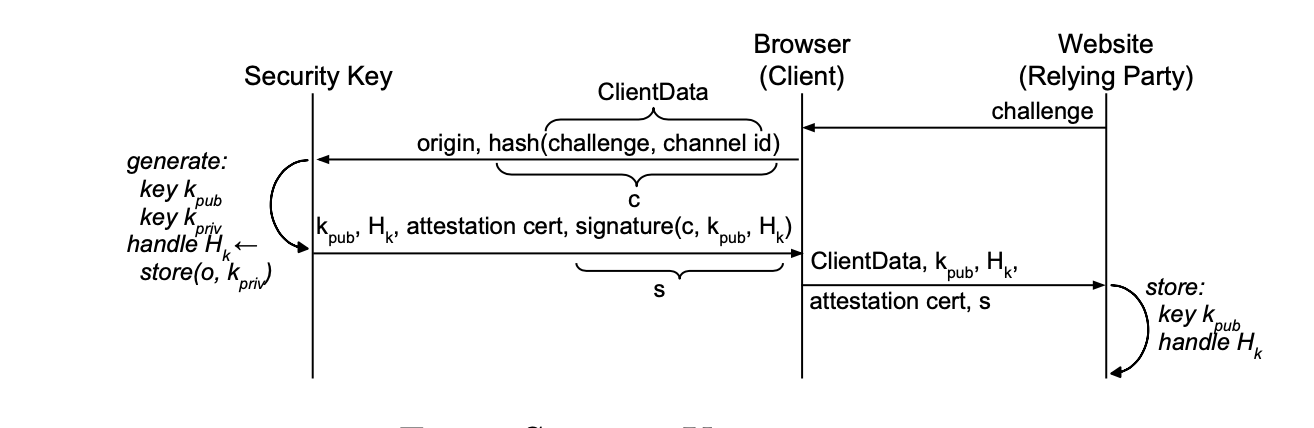
\includegraphics[width=\textwidth]{pics/u2f_reg}
	\caption[\gls{u2f} registration process]{\gls{u2f} registration process\footnotemark}
	\label{fig:u2f_reg}
\end{figure}
\footnotetext{source:...}

A requirement of the registration process of a \gls{u2f} token is that the user already is registered by the \gls{rp}, the web server. The registration process is similar to the introduced process of the \gls{uaf} protocol and also displayed in \autoref{fig:u2f_reg}. At first, the server generates a challenge for the client and sends it along with the username and its AppID to the client, in this case the web browser. The payload also contains the desired version of the \gls{u2f} protocol and the already registered keys, if any. The client again can verify that the AppID matches the origin it is communicating with.

Further, the challenge parameters are constructed by hashing \textit{client data}, i.e., the challenge, AppID, and typ. This data is sent along with the hash of the AppID to the \gls{u2f} token. After that, the token optionally verifies the presence of the user and generates a new public-private key pair over the \gls{nist} \gls{ec} P-256 and stores it with the username. The token sends the \textit{registration data} consisting of the public key, i.e. an uncompress point on the curve and the key handle, which can be wrapped, i.e., encrypted, back to the client. In addition, the attestation certificate of the token and an \gls{ecdsa} signature over the values hashed AppID, hashed challenge, key handle, and pubic key are sent back to the client.

Finally, the client forwards the registration and client data to the \gls{rp}, which can cryptographically verify the data by the signature and attestation certificate.

The following \autoref{listing:u2f_reg} shows the high-level \gls{api} JavaScript registration process.
\\
\begin{example}{Example U2F registration code}
\begin{minted}[breaklines]{javascript}
const registerRequest = {
  challenge: 'Wings2019', // normally is a random string
  version: 'U2F_V2' // where V2 refers to protocol version 1.2
  appId: 'https://timbrust.de'
};

u2f.register('https://timbrust.de', [registerRequest], [], (response) => {
  console.log(response)
});
\end{minted}
\label{listing:u2f_reg}
\end{example}

The challenge value in the \textit{registerRequest} usually is a random challenge and base64 encoded, but for demonstration purposes a plain text string is used instead. In a real world scenario, the \textit{registerRequest} object is generated by the server and sent to the client and the \textit{u2f} JavaScript object is called from the client.

The received response is displayed in \autoref{listing:u2f_reg_resp} and contains the already explained bas64 encoded \textit{registrationData} and the base64 encoded \textit{clientData}. For better readability the strings clientData and registrationData are trimmed. Also, the clientData is decoded to show which data it contains. The client always returns an errorCode \textit{0 (OK)} indicating a successful registration. Other error codes include an other error (1), bad request (2), unsupported configuration (3), ineligible device (4), or timeout (5).

\begin{example}{Example U2F registration response}
\begin{minted}[breaklines]{javascript}
const response = {
  clientData: 'eyJjaGFsbGVuZ2UiOiJXaW5nczIwMTkiLCJvcmlnaW4i [...]', // further data is omitted for readability
  errorCode: 0,
  registrationData: '...', // omitted for readability
  version: 'U2F_V2'
}

// bota() decoded clientData yields
const decodedClientData = {
  challenge: 'Wings2019',
  origin: 'https://timbrust.de',
  typ: 'navigator.id.finishEnrollment'
}
\end{minted}
\label{listing:u2f_reg_resp}
\end{example}

Further the clientData consists of \textit{typ} with the value \textit{navigator.id.finishEnrollment} for a successful registration as well as the challenge of the \gls{rp} and the origin.

\subsubsection{Authentication}

The authentication involves signing a challenge the \gls{rp}, the web server, sends with the corresponding private key, in order that the \gls{rp} can cryptographically verify the the response with the saved public key. \autoref{fig:u2f_auth} shows the procedure, too. The \gls{rp} begins by sending a random challenge, the key handle associated with the user, and the AppID to the client. As in the registration phase, the client can verify the received AppID.

Afterwards, the challenge parameters (hash of the client data) are constructed by hashing the challenge, AppID, and typ. This data is sent along with the hash of the AppID to the \gls{u2f} token. There is no difference in this process compared to the registration

Upon reception, the \gls{u2f} token verifies the presence of the user and retrieves the stored key-pair associated with the key handle.	It sends the counter, that is increased by each usage, and the \gls{ecdsa} over the values user presence, counter, challenge parameters and the hash of the AppID back to the client.

The client forwards registration dat, client data, and key handle to the \gls{rp}, which in return can verify the signature data with the stored public key.

\begin{figure}[hbt]
	\centering
	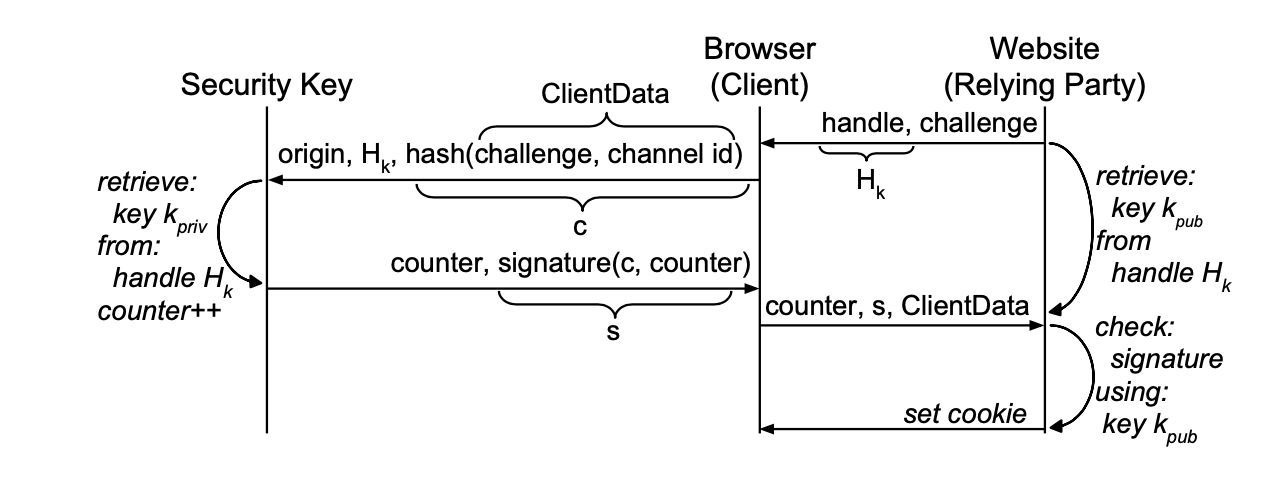
\includegraphics[width=\textwidth]{pics/u2f_auth}
	\caption[\gls{u2f} authentication process]{\gls{u2f} authentication process\footnotemark}
	\label{fig:u2f_auth}
\end{figure}
\footnotetext{source:...}

The \autoref{listing:u2f_reg} shows an example, high-level \gls{api} JavaScript signing process. The \gls{rp} sends the associated key handle, the protocol version, AppID and authentication challenge to the client. \autoref{listing:u2f_auth_resp} shows the generated response by the \gls{u2f} token. The response object and decoded client data shows the \autoref{listing:u2f_auth_resp}.
\\
\begin{example}{Example U2F authentication code}
\begin{minted}[breaklines]{javascript}
const registeredKey = {
  keyHandle: '_WFf5BJ1dwtSCFzfWHoqKUhc9M3Hi0Tv58LAtPz0qM6B3A [...]', // further data is omitted for readability
  version: 'U2F_V2'
}

u2f.sign('https://timbrust.de', 'Wings2019Auth', [registeredKey], [], (response) => {
    console.log(response)
  }
)
\end{minted}
\label{listing:u2f_auth}
\end{example}

\begin{example}{Example U2F authentication response}
\begin{minted}[breaklines]{javascript}
const response = {
  clientData: 'eyJjaGFsbGVuZ2UiOiJXaW5nczIwMTlBdXRoIiwib3JpZ2H [...]', // further data is omitted for readability
  errorCode: 0,
  keyHandle: 'WFf5BJ1dwtSCFzfWHoqKUhc9M3Hi0Tv58LAtPz0qM6B3A-iT [...]', // further data is omitted for readability
  signatureData: 'AQAAAhIwRQIhAK7xli8pV2cc8TKTOYMcdiz-ZuNVes [...]', // further data is omitted for readability
}

// bota() decoded clientData yields
const decodedClientData = {
  challenge: 'Wings2019Auth',
  origin: 'https://timbrust.de',
  typ: 'navigator.id.getAssertion'
}
\end{minted}
\label{listing:u2f_auth_resp}
\end{example}

The client sends back the client data, not its hash, the error status, as well as the key handle and the signature data, signed with the private key. The decoded client data shows again the origin and challenge and a new value for type of operation, in this case \textit{getAssertion}.

\footcites[See][1--2, 4]{u2f-overview}[See][4]{u2f-js-api}